\documentclass[
nopagebreaks,
style=klope,
fleqn]{powerdot}
\usepackage{amsmath, amsfonts}
\usepackage{hyperref}
\usepackage{breakurl}
\usepackage{paralist}
\usepackage{subfig}
\usepackage{algpseudocode}
\usepackage{algorithmicx}
\usepackage{algorithm}
\title{K-Means Clustering}
\author{Yige Hu and Zhiting Zhu}
\date{}

\begin{document}

\maketitle

% declaration of the new block
\algblock{ParFor}{EndParFor}
% customising the new block
\algnewcommand\algorithmicparfor{\textbf{parfor}}
\algnewcommand\algorithmicpardo{\textbf{do}}
\algnewcommand\algorithmicendparfor{\textbf{end\ parfor}}
\algrenewtext{ParFor}[1]{\algorithmicparfor\ #1\ \algorithmicpardo}
\algrenewtext{EndParFor}{\algorithmicendparfor}

\algnewcommand\algorithmicinput{\textbf{INPUT:}}
\algnewcommand\INPUT{\item[\algorithmicinput]}

\begin{slide} {Problem}
  \begin{compactitem}
  \item{Input: a set of data points $\{x_i|i = 1..n\} \subseteq
    \mathbb{R}^d $}
  \item{Task: partition the n data points
    in to k($\leq n$) sets S = $\{S_1, S_2, ..., S_k\}$ so as to minimize
    the within-cluster sum of squared
    errors, $$\arg\min_{S}\sum_{i=1}^{k}\sum_{x \in S_i} \parallel x -
    \mu(S_i)\parallel$$ where $\mu(S_i)$ is the mean of points in $S_i$}
  \item{NP-hard problem for global optimal solution
    \begin{compactitem}
    \item{In general d dimention Euclidean space even with 2 clusters}
    \item{k clusters in the same plane}
    \end{compactitem}
  }
  \item{Heuristic algorithm}
  \end{compactitem}
  \vspace{-0.6in}
  \begin{figure}
    \flushright
    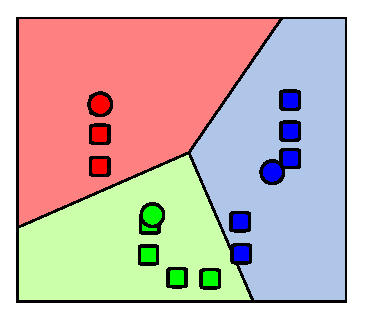
\includegraphics[scale=.5]{fig/K_Means_Example_Step_4.eps}
  \end{figure}
\end{slide}

\begin{slide} {Sequential Algorithm}
  \begin{algorithmic}[1]
    \INPUT k: Number of clusters. N: number of d dimention data points. dp: data points 
    \Function{seq\_k-means}{dp, N, k}
    \State Randomly generate k points as cluster centers
    \State Assign each point to the nearest cluster center
    \State Recompute the new cluster centers
    \State Repeat the previous two steps until some convergence criterion
    is met
    \EndFunction
  \end{algorithmic}
  \begin{compactitem}
    \item{Suppose the algorithm runs m iterations. Time complexity: O(Nkdm)}
  \end{compactitem}
\end{slide}

\begin{slide} {Sequential Algorithm}
  \begin{figure}[h]
    \centering
    \subfloat[t][~\cite{f1}]{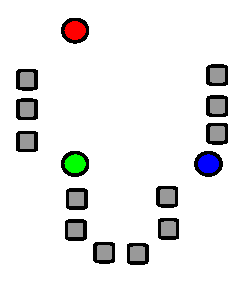
\includegraphics[scale=.5]{fig/K_Means_Example_Step_1.eps}}\qquad
    \subfloat[t][~\cite{f2}]{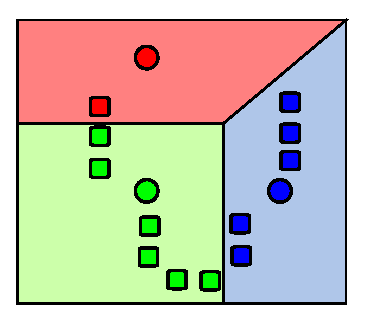
\includegraphics[scale=.5]{fig/K_Means_Example_Step_2.eps}}\\
    \subfloat[t][~\cite{f3}]{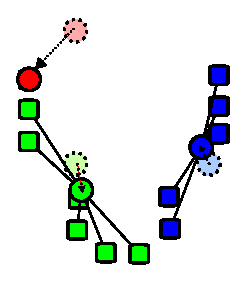
\includegraphics[scale=.5]{fig/K_Means_Example_Step_3.eps}}\qquad
    \subfloat[t][~\cite{f4}]{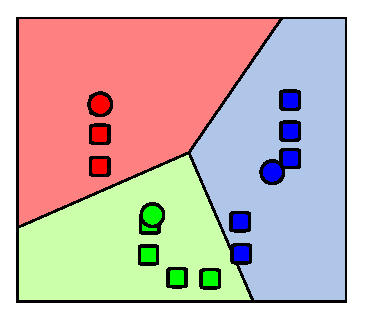
\includegraphics[scale=.5]{fig/K_Means_Example_Step_4.eps}}
  \end{figure}
\end{slide}

\begin{slide} {Parallel Algorithm}
  \footnotesize
  \begin{algorithmic}[1]
    \INPUT k: Number of clusters. N: number of data points. d: data points
    \Function{par\_k-means}{d, N, k} \label{alg:p}
    \State Partition N data objects evenly among all threads
    \State Randomly choose k points as cluster mean
    \While {!(converges with respect to a threashold) and (iterations
      $<$ MAX\_ITERATIONS)}
    \ParFor {t = 1..p}
    \State calculate the distance between each point and
    cluster centroids
    \State find the nearest centroid
    \State change membership according to the new centroid
    \State calculate the new centroid of each cluster
    \EndParFor
    \State Calculate differences between new membership assignment and
    old membership assignment
    \EndWhile
    \EndFunction  
  \end{algorithmic}
\end{slide}

\begin{slide}{Goal}
  \begin{compactitem}
    \item{Implement parallel algorithm in CUDA. GPU specific optimization}
  \end{compactitem}
\end{slide}

\begin{slide} {References}
\footnotesize
\bibliographystyle{acm}
\bibliography{bibliography}
\end{slide}
\end{document}
